\section{Neo4j} \label{Chap:Neo4j}
As a persistent backend storage, it has been decided to use Neo4j \cite{neo4j}. The main reasons behing this choice are:
\begin{itemize}
  \item ease of use;
  \item a graph database is very handy when working with maps;
  \item neo4j is the leader in the development of graph database frameworks.
\end{itemize}
The developed library for interfacing with the database is located in package \textit{it.polito.dp2.rest.rns.neo4j} and it is based on the usage of Neo4j drivers and Cypher query language, that is one of the two way to go suggested by Neo4j documentation (Cypher and drivers \cite{neo4jcypher} or HTTP rest API \cite{neo4jhttprest}). \\
The package contains two classes:
\begin{enumerate}
  \item class \textbf{Neo4jInteractions.java}: it is used to to start/close a session with the database, execute a query, retrieve the results. It basically offers a set of function to allow the service layer of the server application to store, retrieve, delete and update data;
  \item class \textbf{StatementBuilder.java}: this class is responsbile of providing a set of functions that create statements (a.k.a. queries), to be run in the database through the driver, depending on some parameters that are given.
\end{enumerate}
The access from service layer to database layer is achieved through an object of type \textbf{Neo4jInteractions}. It has been developed using a \textit{singleton} pattern in order to have only one instance of this object for the whole application. Such pattern consists in the definition of a private constructor and a private static instance of an object of the same type of the containing class. This is instance is made accessible through static methods. \\
In the database, each neo4j node corresponds to a place. Since the defined model for the project stated that even connection between places are to be considered places themselves, the relationships between nodes that neo4j offers have been exploited in a different way. What relationships have been used is to describe two things:
\begin{enumerate}
  \item the \underline{type} of relationship existing between the nodes (container, connection, ...);
  \item the \underline{direction} in which is possible to traverse the two nodes. Let's assume there exist two nodes, \textit{node1} and \textit{node2}, that are strongly connected (which means there is a relationship from \textit{node1} to \textit{node2} and one the other way around), a vehicle is able to go either from \textit{node1} to \textit{node2} or from \textit{node2} to \textit{node1}. If there is only one relation, for instance from \textit{node1} to \textit{node2}, the vehicle will only be able to traverse the nodes the same direction the relation is pointing (in this case \textit{node1}$\rightarrow$ \textit{node2}).
\end{enumerate}
\begin{figure}[!htb]
   \centering
   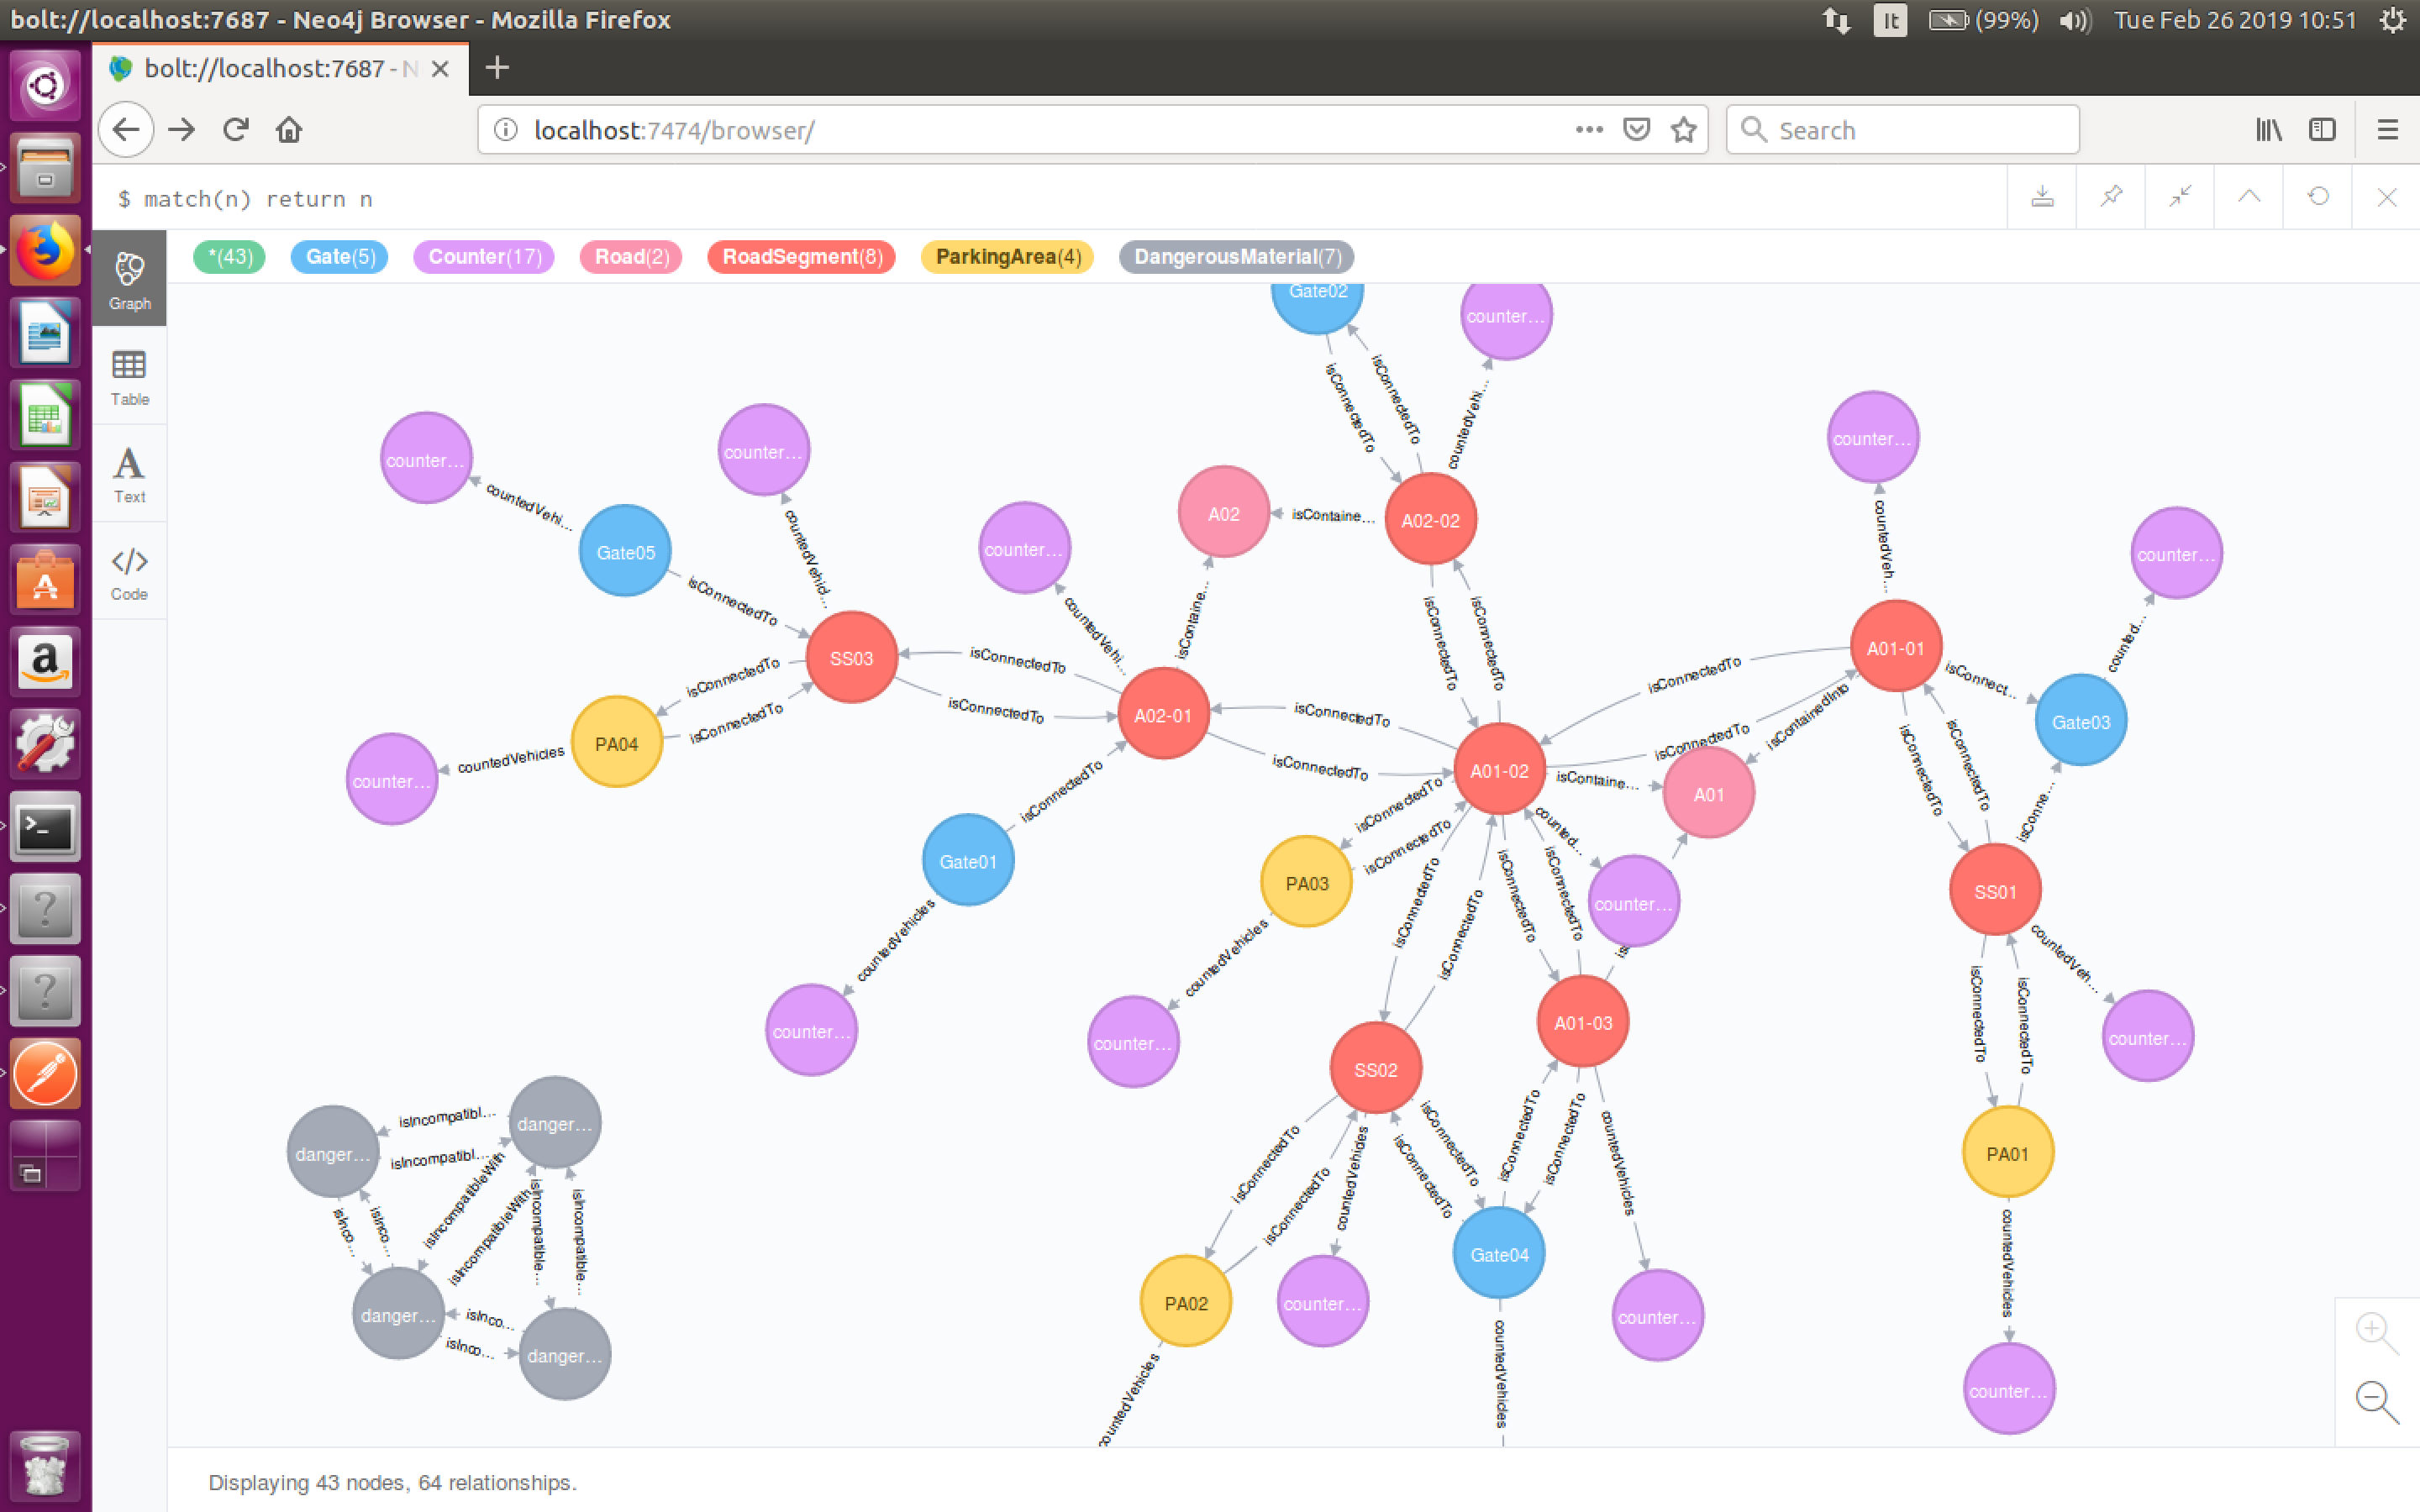
\includegraphics[width=\textwidth]{neo4j_graph.png}
   \caption{Example of graph of the system.}\label{Fig:Neo4jGraph}
\end{figure}
In figure \ref{Fig:Neo4jGraph}, it is represented a possible description of a system where there are present gates, parking area, road segments and road. Other than that, worth of a notice is the presence of some particular nodes:
\begin{itemize}
  \item \textbf{counter} nodes (\textit{purple} nodes in figure \ref{Fig:Neo4jGraph}): this kind of nodes are used to track information about places. There is a counter node for each place and it is responsible of keeping the number of reservations for that place and the number of vehicles that have passed through that place;
  \item \textbf{dangerous material} nodes (\textit{gray} nodes in figure \ref{Fig:Neo4jGraph}): it is present a node, for each dangerous material known by the system. Between these nodes exist relations of incompatibility, in order to allow the system to recognize if a material is incompatible with another.
\end{itemize}
